%!TEX encoding=UTF-8
\documentclass[ 4paper,11pt,openany]{book}
\usepackage[T1]{fontenc}
\usepackage[english,italian]{babel}
\usepackage{graphicx}
\usepackage[margin=1in]{geometry}
\usepackage{listings}
\usepackage{xcolor}
\usepackage{hyperref}

\title{Progetto Lavoratori Stagionali}
\author{Ledjo Lleshaj VR450678\\Silver Gjeka VR450793}
\date{Anno 2021/2022}

\begin{document}
\frontmatter
\maketitle
\tableofcontents 

\mainmatter
\chapter{Introduzione}
\section{Consegna}
Si vuole progettare un sistema informatico di una agenzia che fornisce servizi di supporto alla ricerca di lavoro stagionale. I lavoratori interessati possono iscriversi al servizio, rivolgendosi agli sportelli dell’agenzia. Il sistema deve permettere la gestione delle anagrafiche e la ricerca di lavoratori
stagionali, nei settori dell’agricoltura e del turismo. 

I responsabili del servizio, dipendenti dell’agenzia, inseriscono i dati dei lavoratori. 
Per ogni lavoratore vengono memorizzati i dati anagrafici (nome, cognome, luogo e data di nascita, nazionalità), indirizzo, recapito telefonico personale (se presente), email, le eventuali
specializzazioni/esperienze precedenti (bagnino, barman, istruttore di nuoto, viticultore,floricultore), lingue parlate, il tipo di patente di guida e se automunito. Sono inoltre memorizzati i periodi e le zone (comuni), per i quali il lavoratore è disponibile. Di ogni lavoratore si memorizzano anche le informazioni di almeno una persona da avvisare in caso di urgenza: nome, cognome, telefono, indirizzo email. 

I dipendenti dell’agenzia devono autenticarsi per poter accedere al sistema e inserire i dati dei lavoratori. Il sistema permette ai dipendenti dell’agenzia di aggiornare le anagrafiche con tutti ilavori che i lavoratori stagionali hanno svolto negli ultimi 5 anni. 
Per ogni lavoro svolto vanno registrati: periodo, nome dell’azienda, mansioni svolte, luogo di lavoro, retribuzione lorda giornaliera. Per i dipendenti dell’agenzia si memorizzano i dati anagrafici, l’indirizzo email, il telefono e le credenziali di accesso (login e password).

Una volta registrate le informazioni sui lavoratori, il personale dell’agenzia può effettuare ricerche rispetto a possibili profili richiesti.
In particolare, il sistema deve permettere ai dipendenti di effettuare ricerche per lavoratore, per lingue parlate, periodo di disponibilità, mansioni indicate, luogo di residenza, disponibilità di auto/patente di guida. Il sistema deve permettere di effettuare ricerche complesse, attraverso la specifica di differenti condizioni di ricerca (sia in AND che in OR).
 \pagebreak


\section{Metodologia di lavoro adottata}
La metodologia di lavoro da noi adottata si avvicina molto al modello plan driven, infatti tutte le attività del processo sono state pianificate in anticipo secondo un modello a cascata che prevedeva l'analisi iniziale dei requisiti, la progettazione del software da un punto di vista ad alto livello, la realizzazione dello stesso tramite il linguaggio di typescript e Vue per la parte di Frontend e python con framework Django e database SQLite e una fase finale di test per verificare la corretta funzionalità del prodotto finale.
Questa metodologia di sviluppo è stata usata maggiormente nella parte di sviluppo dell'interfaccia grafica e di tutta la parte relativa ai controlli gestiti da quest'ultima, la parte del progetto riguardante la gestione dei dati (memorizzazione lettura ecc.) è stata ideata seguendo una mista strategia di metodo agile con pianificazione incrementale e a volte di Test Driven Development per i componenti vari. Il lavoro è stato gestito con la metodologia scrum, i compiti da eseguire erano principalmente suddivisi in compiti riguardanti il frontend(Vuejs/Typescript/) e compiti riguardanti il backend(Python/Django-Sqlite). 
Il lavoro e la condivisione del progetto sono stati gestiti grazie al software di controllo di versione git e GitHub che permette di lavorare in gruppo in maniera efficiente anche modificando il progetto in maniera asincrona (su branch differenti) per poi combinare le diverse modifiche (merge) fatte in un secondo momento, per questo non è stato necessario incontrarsi spesso per decidere come procedere col lavoro.  Di seguito è riportato un breve schema che riassume la divisione dei lavori, a sinistra il nome e a destra la lista dei compiti svolti. \href{https://github.com/Job-Searching-Webpage}{Github repos}
\clearpage


\chapter{Struttura del progetto}
In questo capitolo sarà descritta la struttura generale del progetto e come esso si presenta all'utente finale. Verranno poi mostrati alcuni esempi di casi d'uso principali con relativi diagrammi di sequenza, per concludere sarà mostrato un diagramma riassuntivo delle attività generali.


\section{Casi d'uso principali}
Il diagramma dei casi d'uso raffigurato qui sotto mostra i modi principali per utilizzare questa applicazione, di seguito sono riportati i singoli casi d'uso descritti più nel dettaglio.
\begin{figure}[htpb!] 
	\subsection{Diagrama dei Casi d'uso}
	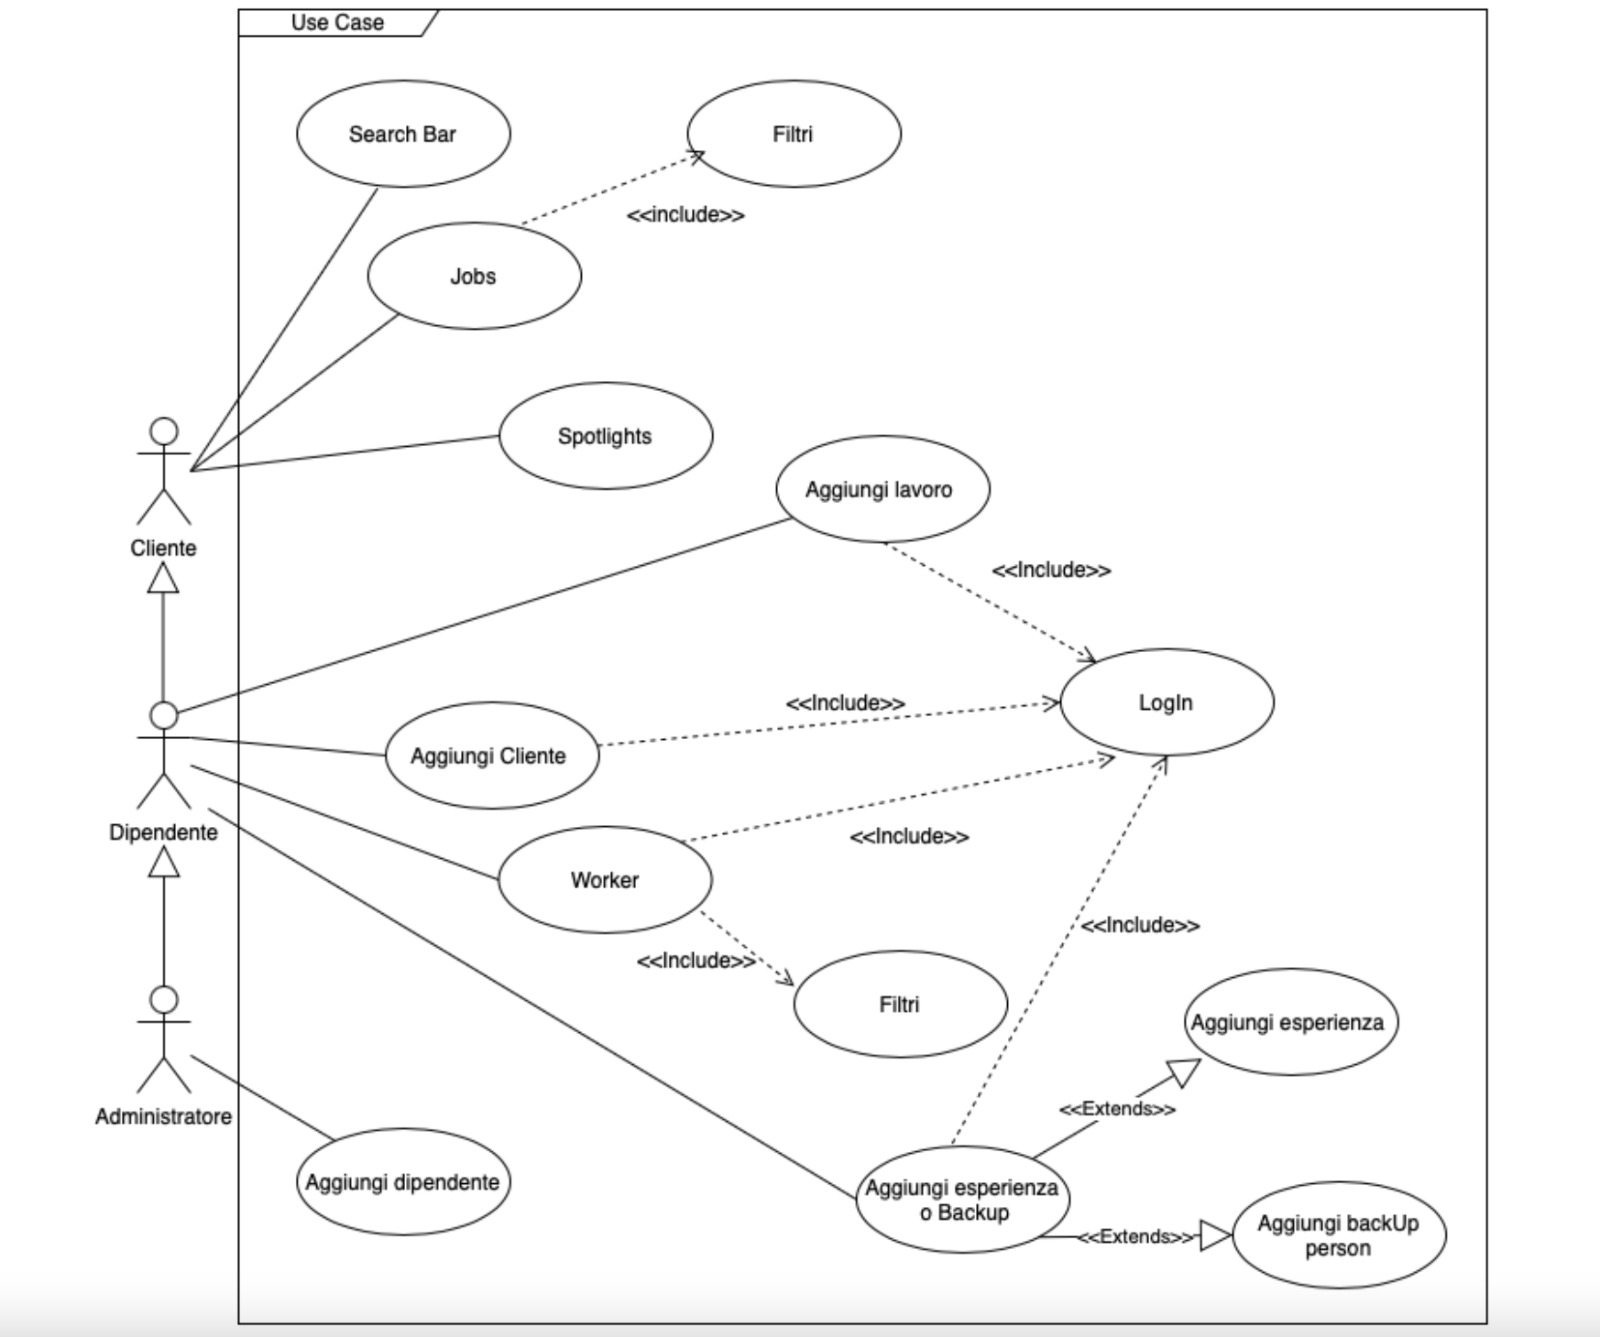
\includegraphics[height=190mm,width=180mm]{UseCase.jpeg}
\end{figure}


\subsection{Registrazione di un lavoratore con rispettiva esperienza lavorativa TO DO SILVER}
\textbf{Precondizioni}: l'utente deve essere autenticato\\
\textbf{Attore}: Dipendente (può essere anche l'amministratore)\\
\textbf{Passi}:
\begin{enumerate}
\item Il dipendente registra un nuovo lavoratore
\item Il dipendente cerca il lavoratore appena creato, apre la sua pagina di modifica 
\item Il dipendente aggiunge una nuova esperienza lavorativa tramite la pagina di modifica del lavoratore
\end{enumerate}
\textbf{Postcondizioni}: un nuovo lavoratore con un'esperienza lavorativa è stato inserito\\

\subsection{Modifica di un lavoratore}
\textbf{Precondizioni}: l'utente deve essere autenticato\\
\textbf{Attore}: Dipendente (può essere anche l'amministratore)\\
\textbf{Passi}:
\begin{enumerate}
\item Il dipendente cerca il lavoratore tramite la pagina di ricerca
\item Il dipendente apre la scheda del lavoratore cliccando sulla tabella 
\item Il dipendente modifica il lavoratore
\item Il dipendente salva le modifiche
\end{enumerate}
\textbf{Postcondizioni}: un lavoratore è stato modificato\\

\subsection{Modifica di un'esperienza lavorativa}
\textbf{Precondizioni}: l'utente deve essere autenticato\\
\textbf{Attore}: Dipendente (può essere anche l'amministratore)\\
\textbf{Passi}:
\begin{enumerate}
\item Il dipendente cerca il lavoratore
\item Il dipendente apre la scheda del lavoratore cliccando sulla tabella
\item Il dipendente apre la scheda con l'elenco delle esperienze lavorative
\item Il dipendente seleziona l'esperienza interessata e la modifica
\item Il dipendente salva le modifiche
\end{enumerate}
\textbf{Postcondizioni}: un'esperienza lavorativa è stata modificata\\

\subsection{Registrazione di un nuovo dipendente}
\textbf{Precondizioni}: l'utente deve essere autenticato come amministratore\\
\textbf{Attore}: Amministratore\\
\textbf{Passi}:
\begin{enumerate}
\item L'amministratore apre la finestra per aggiungere i dipendenti 
\item Registra un nuovo dipendente
\end{enumerate}
\textbf{Postcondizioni}: un nuovo dipendente è stato inserito\\

\section{Diagrammi di sequenza dei casi d'uso}
Qui di sotto sono raffigurati i diagrammi di sequenza dei casi d'uso spiegati in precedenza, è stato scelto di dividere il diagramma in due parti a seconda dell'attore interessato al fine di garantire una maggiore leggibilità. La prima immagine raffigura i passaggi per la creazione e modifica di un lavoratore, la seconda i passi per creare un nuovo dipendente.


\begin{figure}[htpb!] 
\subsection{Diagrama di sequenza dipendenti Completo}
	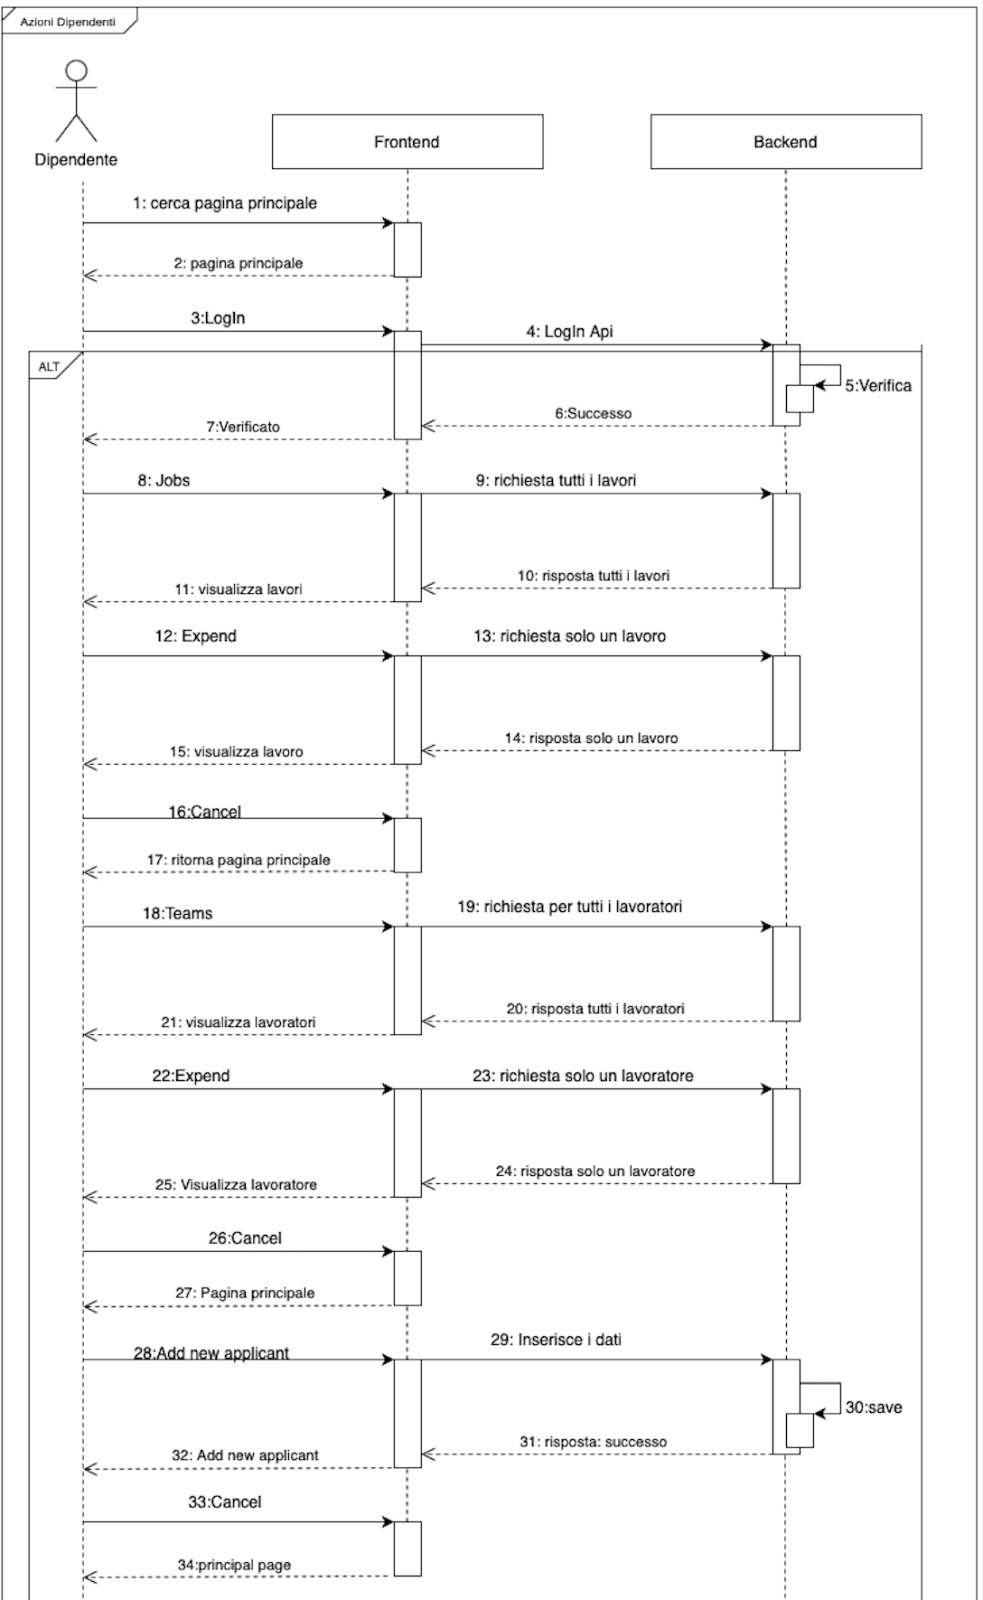
\includegraphics[height=250mm,width=180mm]{Seq_Dipendenti_Completo1.jpeg}
\end{figure}
\begin{figure}[htpb!] 
	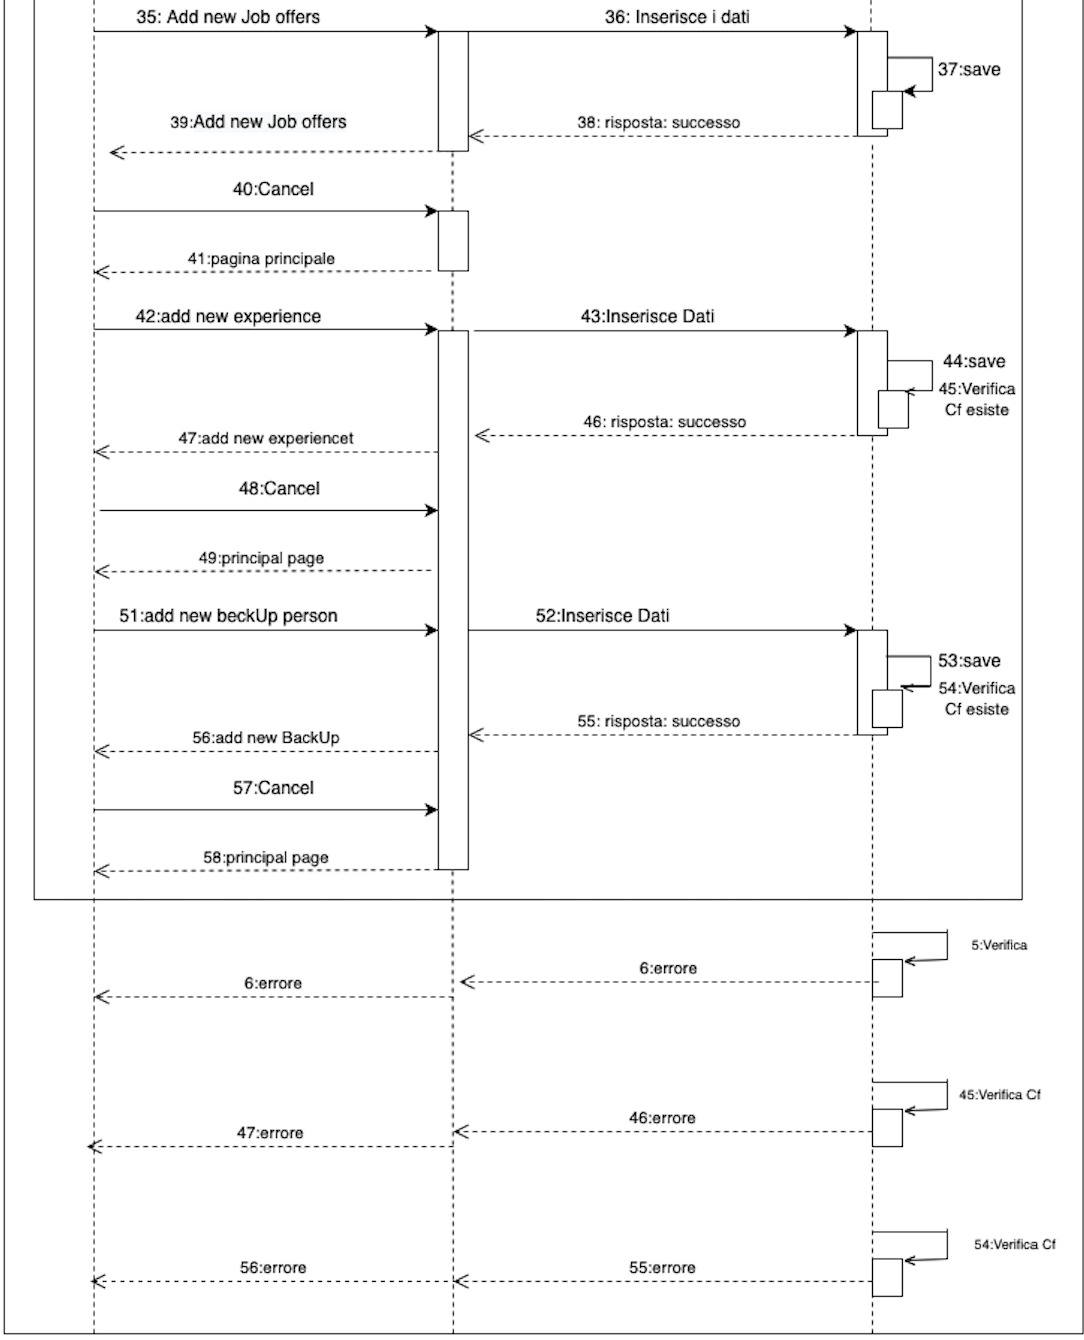
\includegraphics[height=250mm,width=180mm]{Seq_Dipendenti_Completo2.jpeg}
\end{figure}

\begin{figure}[htpb!] 
	\subsection{Diagrama di sequenza user}
	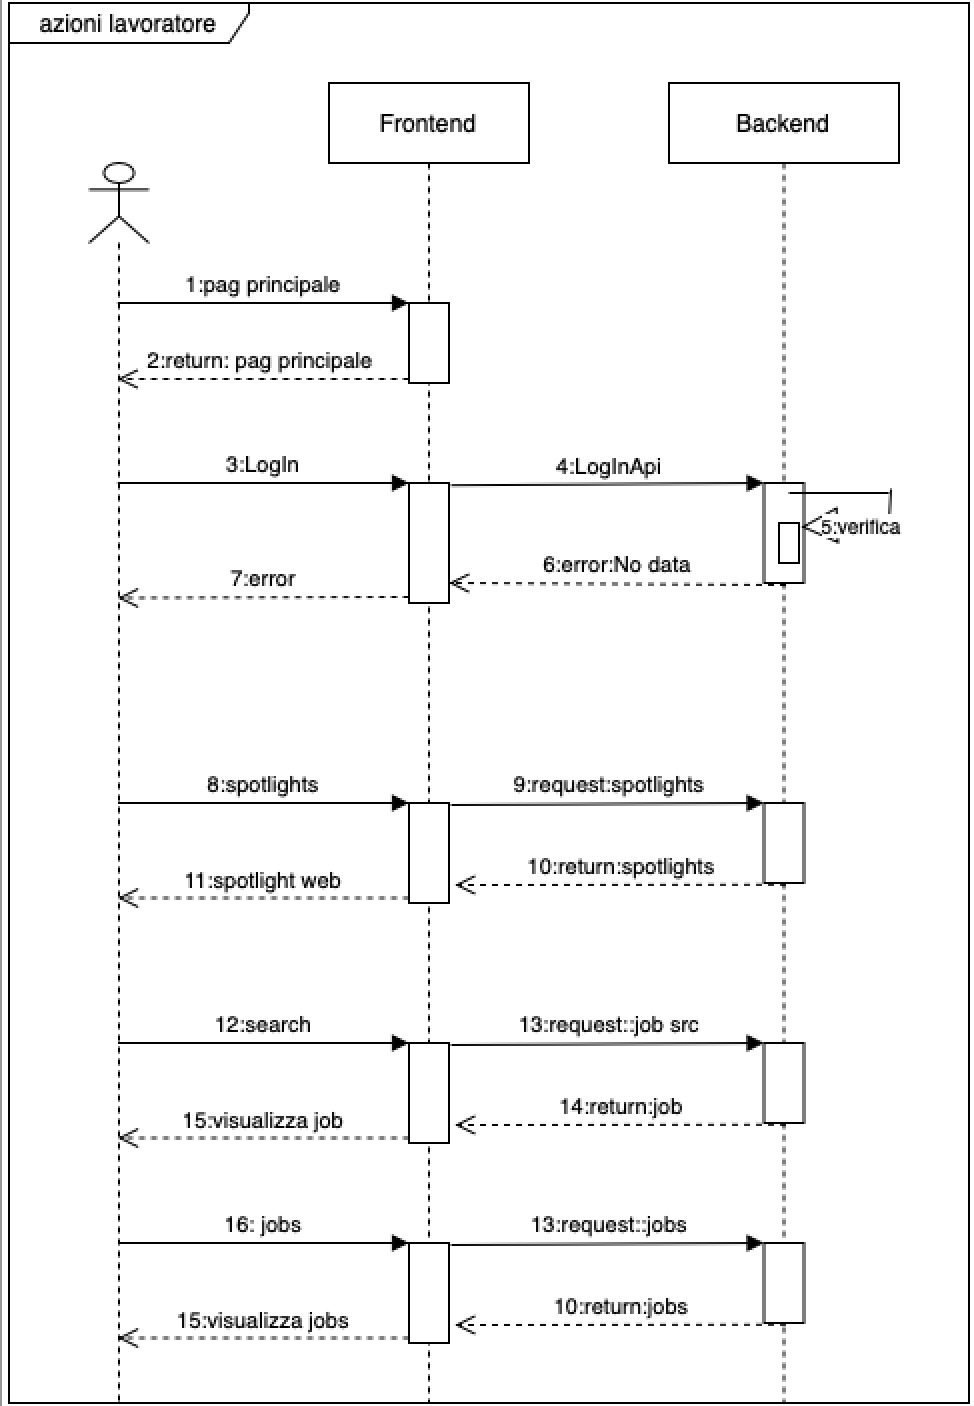
\includegraphics[height=245mm,width=180mm]{Seq_Lavoratore.jpeg}
\end{figure}
\begin{figure}[htpb!] 
	\subsection{Diagrama di sequenza inserimento lavoratore}
	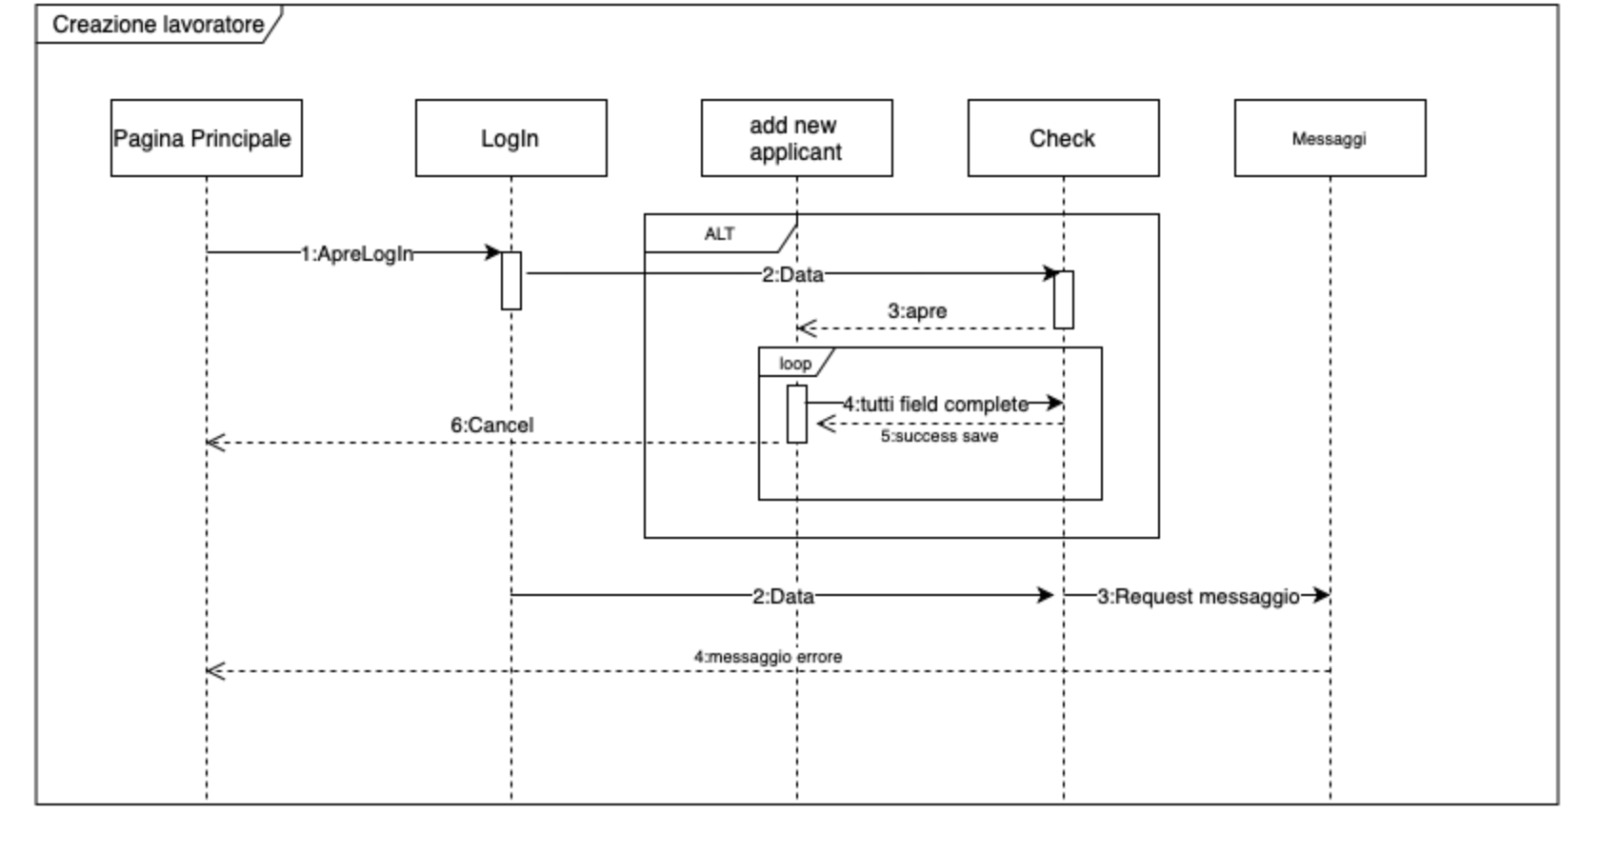
\includegraphics[width=180mm]{creazione_Lavoratore.jpeg}
\end{figure}
\begin{figure}[htpb!] 
	\subsection{Diagrama di sequenza inserimento persona di backup}
	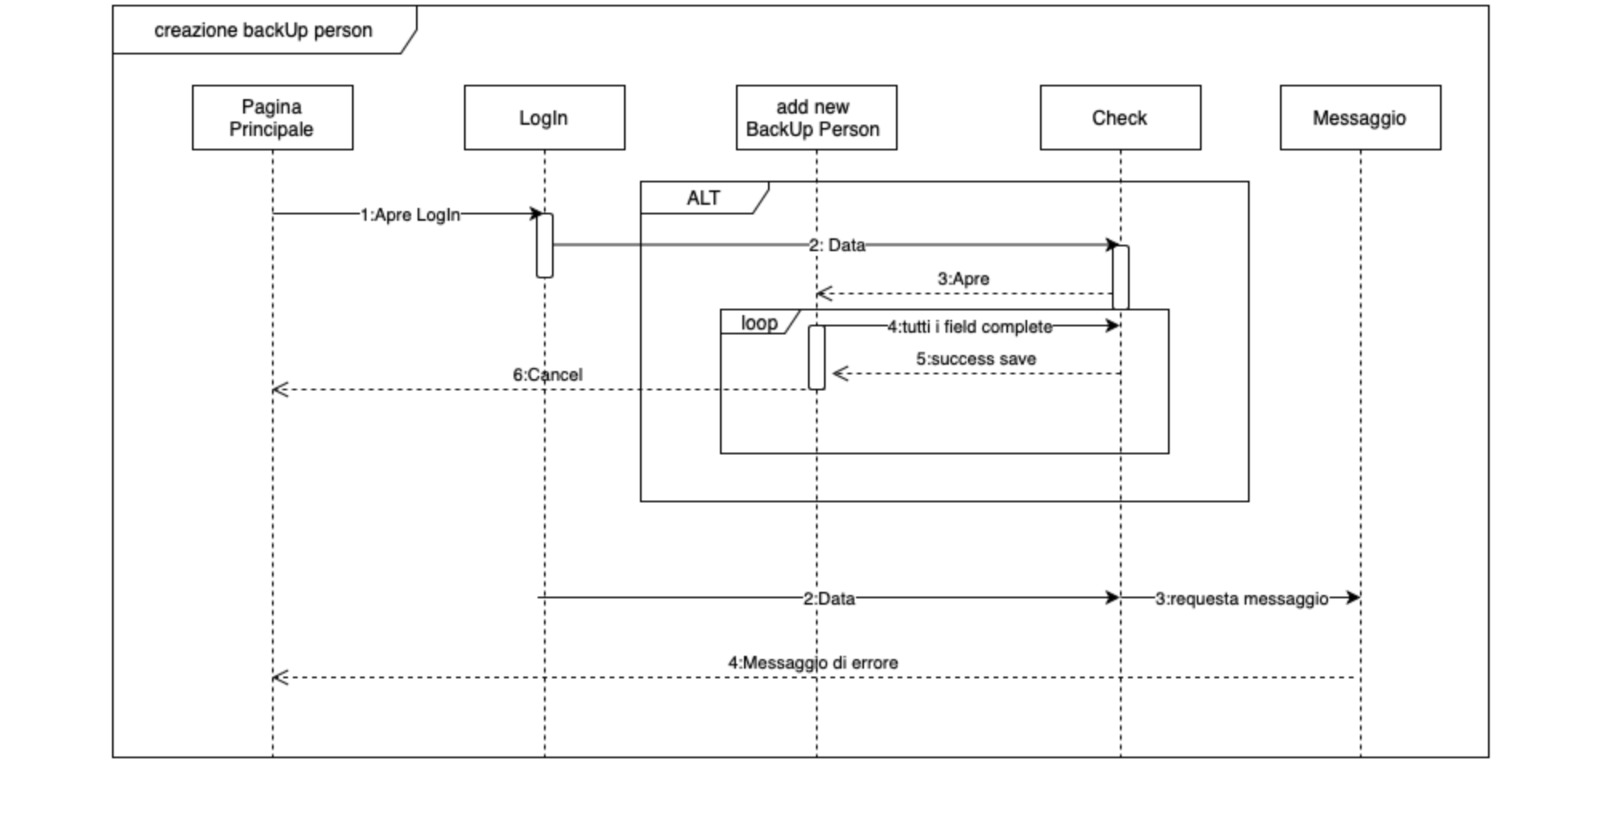
\includegraphics[width=180mm]{creazione_Backup.jpeg}
\end{figure}
\begin{figure}[htpb!] 
	\subsection{Diagrama di sequenza inserimento Experience}
	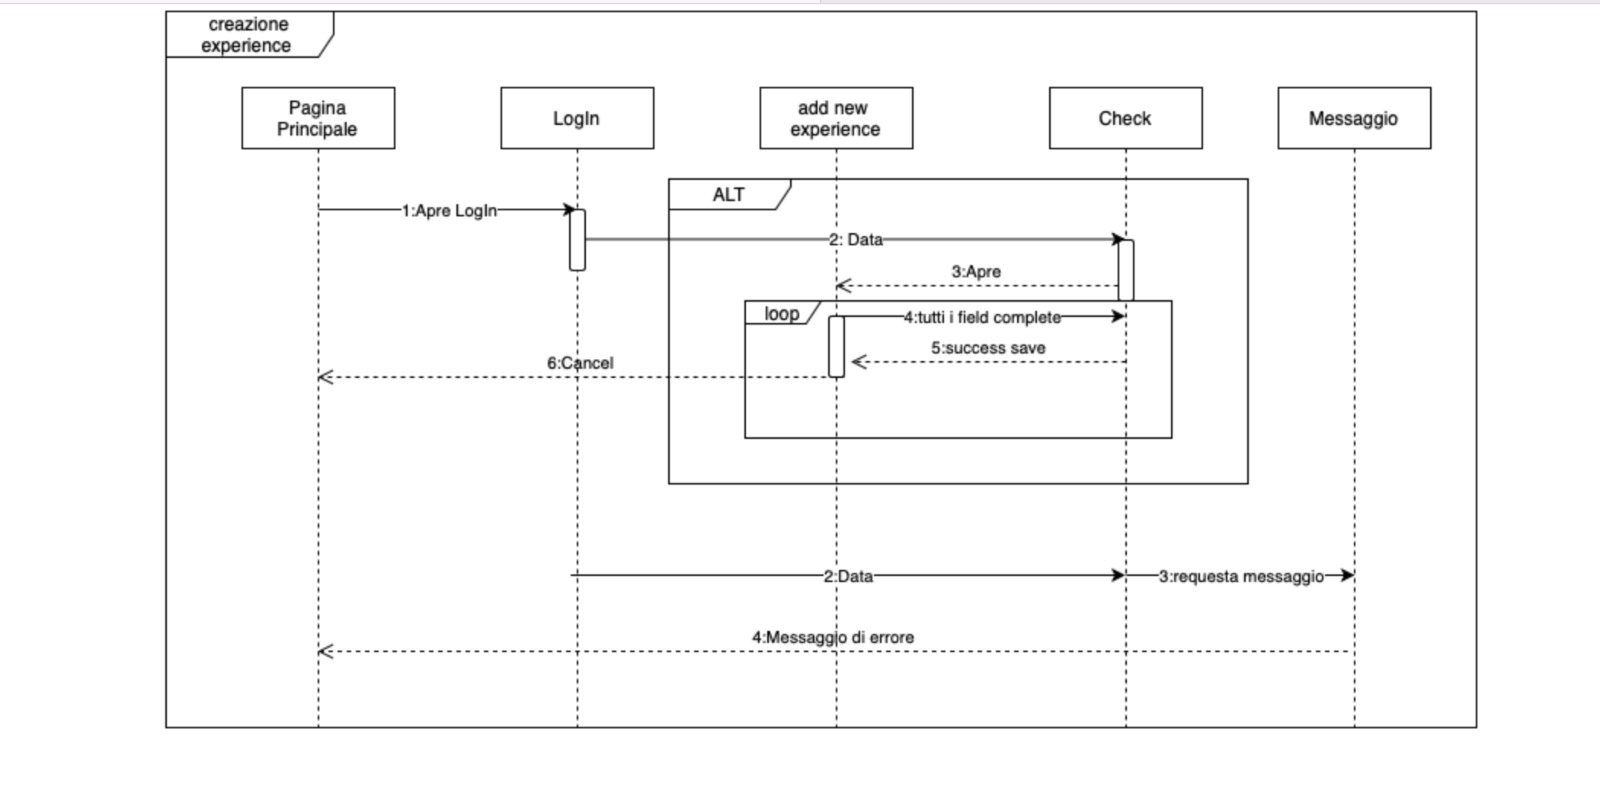
\includegraphics[width=180mm]{creazione_Experience.jpeg}
\end{figure}
\begin{figure}[htpb!] 
	\subsection{Diagrama di sequenza inserimento di oferta di lavoro}
	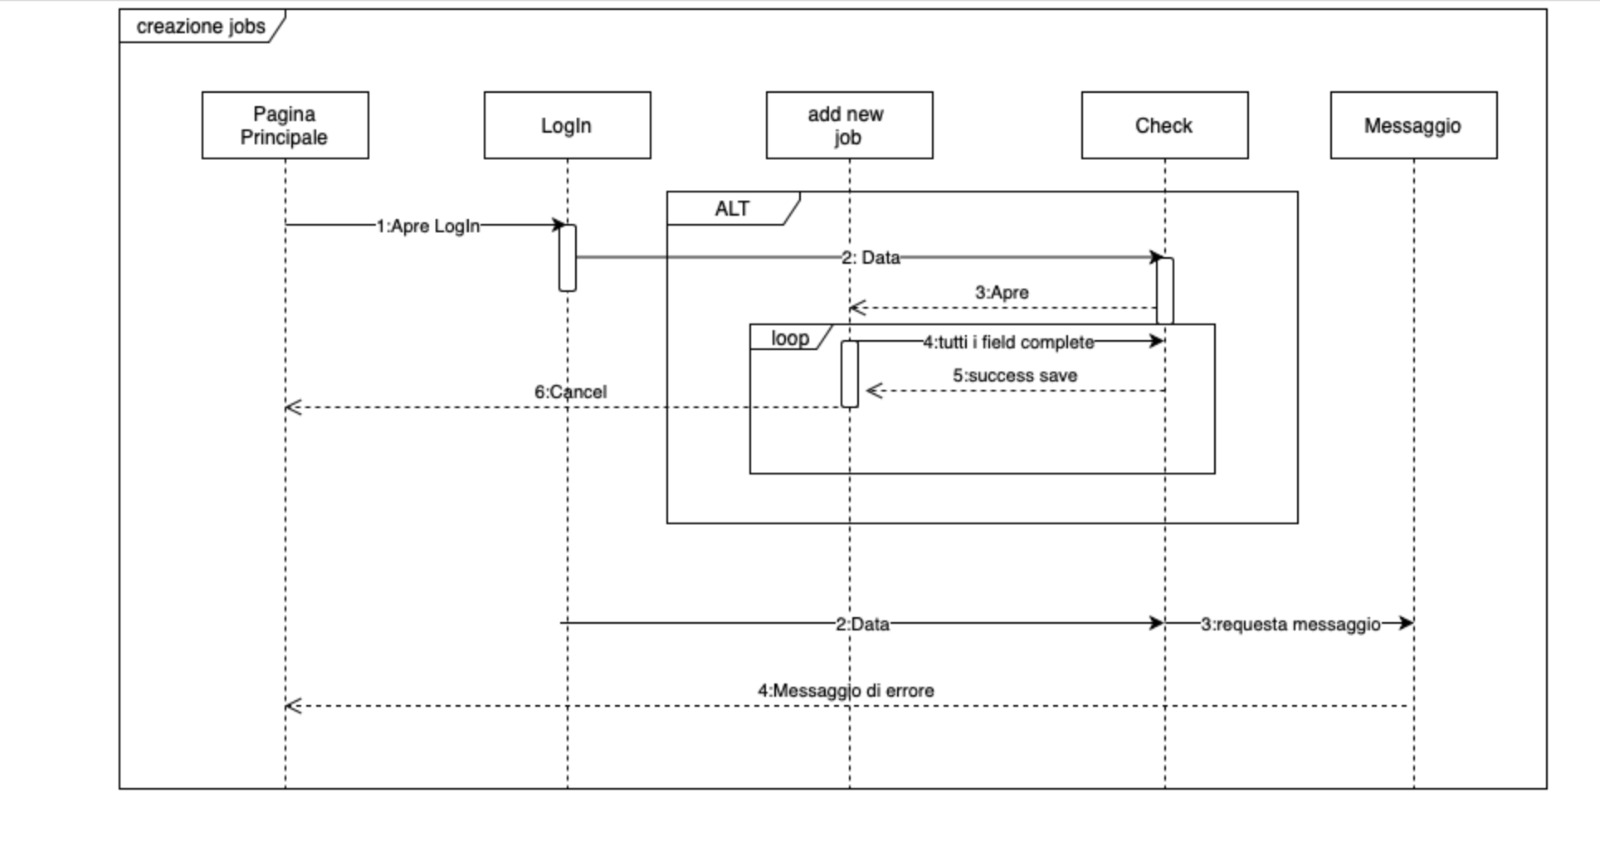
\includegraphics[width=180mm]{creazione_Job.jpeg}
\end{figure}



\chapter{Database}
In questo capitolo verrà trattato tutto ciò che è strettamente legato con il disegno concettuale della diagrama Entita-Relazione e all'implementazione della database relazionale.Verrano inoltre spiegato Django e come interagisce con SQLite.
\section{Database}
\begin{figure}[htpb!] 
	\section{Diagramma Entita-Relazione} 
	\includegraphics[width=185mm]{Database.png}
\end{figure}



\section{SQLite Django To Do Silver}








\chapter{Implementazione}
In questo capitolo verrà trattato tutto ciò che è strettamente legato ai metodi implementativi usati per la realizzazione di questa applicazione. Verranno inoltre descritti i pattern architetturali e di design utilizzati.

\section{Componenti implementati}
Di seguito è riportato un diagramma delle componenti/classi UML dove saranno rappresentate una volta tutte le componenti e in un altra solo le classi utili per far comprendere la struttura generale del progetto, saranno omesse le variabili utilizzate e i metodi, per garantire una migliore leggibilità.

\section{Diagrammi di sequenza del software TODO Silver}
In questa sezione verranno mostrati i diagrammi di sequenza visti in precedenza, dal punto di vista del software progettato. Sono state omesse le parti di registrazione dell'utente per garantire una migliore leggibilità. Le linee di vita sono quelle dei vari componenti che costituiscono l'applicazione, saranno quindi mostrate più in dettaglio le interazioni delle singole parti.
\subsection{Creazione e modifica di un lavoratore}
%\includegraphics[width=180mm]{softwareseq.png}
\subsection{Creazione di un dipendente}
%\includegraphics[width=180mm]{softwareseq2.png}


\begin{figure}[htpb!] 
	\section{Diagramma delle classi/componenti}
	\centering 
	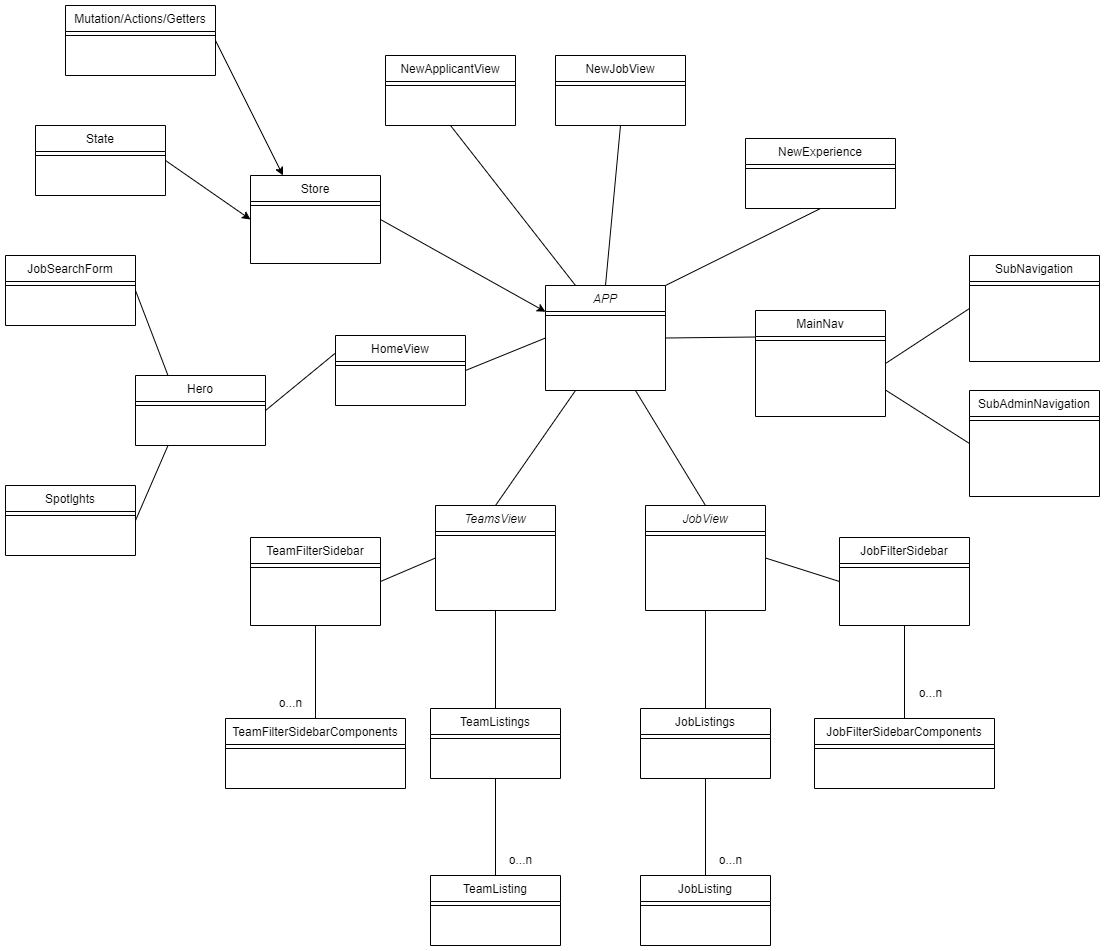
\includegraphics[width=185mm]{Complete_Class_diagram.png}
	Nota: le parti di rappresentazione delle classi riguardanti l'interfaccia grafica e il Management system sono state omesse poichè non fondamentali per capire l'organizzazione dell'applicazione.
\end{figure}


\section{Pattern architetturale: MVVM}
Per scrivere l'applicazione si e' deciso di implementare il pattern architetturale Model~View~Controller (MVC).
E' stato utilizzato il pattern MVC perche' permettere di separare le responsabilita' dell'applicazione in tre parti:
\begin{itemize}
    \item Model: il modello e' la logica interna della applicazione. Questa parte gestisce il login, l'inserimento, la ricerca e l'eliminazione dei dati, la lettura e la scrittura dei dati in modo permanente su disco.
    \item View: la vista e' la parte grafica che gestisce cio' che e' visibile dall'utente. Attraverso questa View e possibile a prendere l'input dall'user. Il contenuto di View non si puo cambiare dall'user.
    \item ViewModel: si trova tra Model e View e gestisce l'interazione dell'utente con l'interfaccia grafica permettendo la comunicazione tra la vista e il modello tramite Binding tra la UI in View e i controlli in Model.
\end{itemize}
\begin{center}
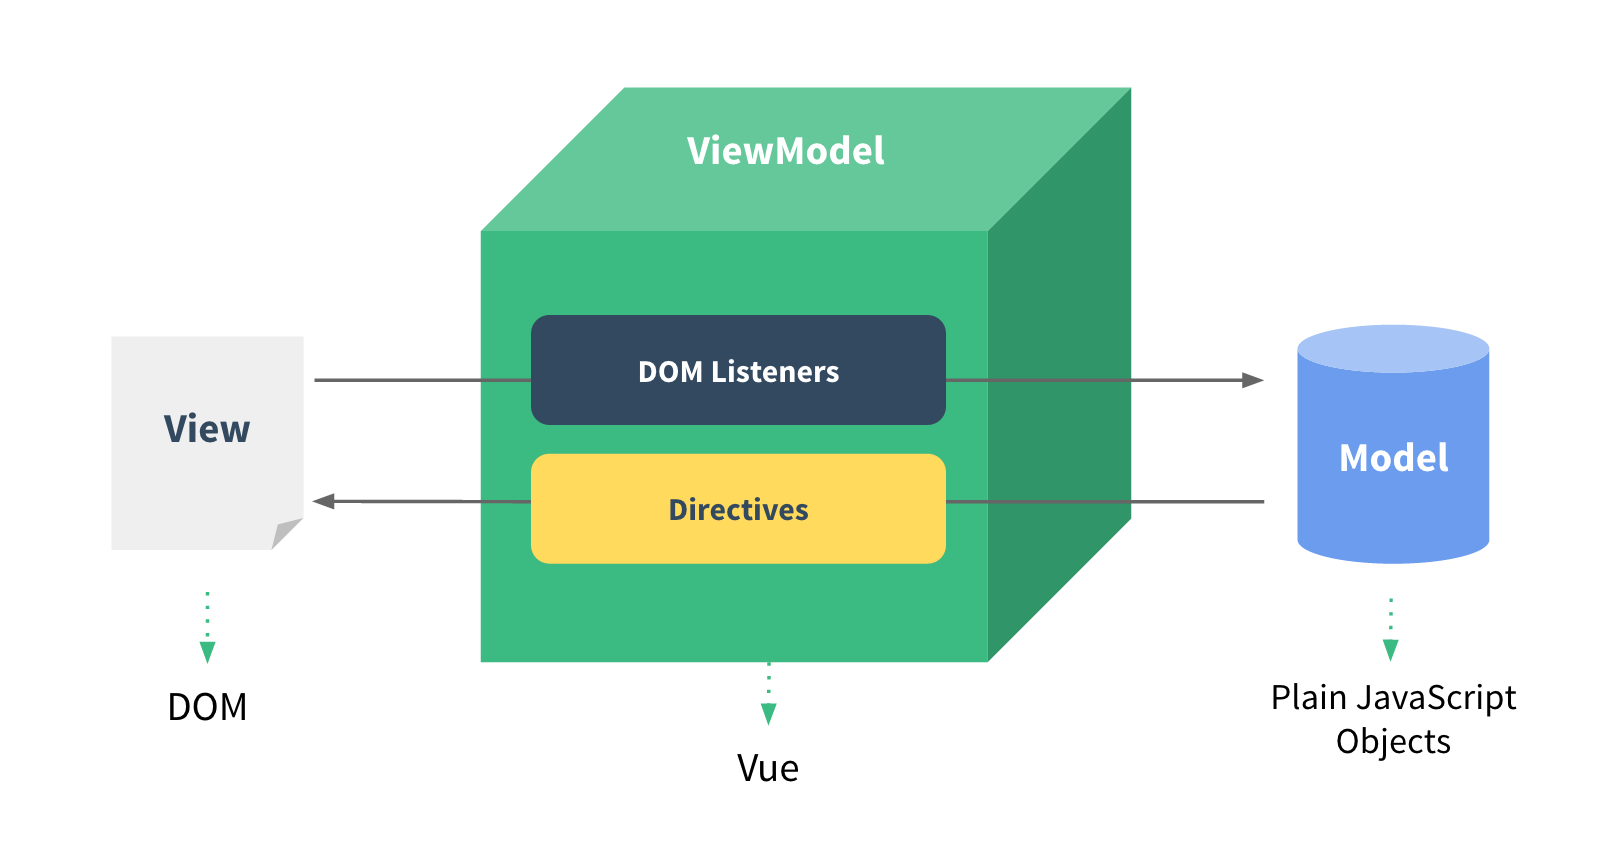
\includegraphics[width=170mm]{Vuemvvm.png}
\end{center}

\section{Pattern di design: Singleton}
Per gestire il funzionamento corretto della pagina e' stata creata una classe chiamata Store che contiene oggetti seguendo il pattern Singleton.Un particolare esempio e Lo state che contiente un oggetto globale chiamato globalState.
Il pattern Singleton garantisce che all'interno della applicazione venga creata una sola istanza di questa classe.

Il vantaggio del pattern singleton applicato a questo approccio è che permette di poter richiedere facilmente l'istanza all'interno di un qualsiasi controller garantendo che non sarà mai possibile avere stati indeterminati o multipli del sistema: è sempre presente un unico stato che evolve nel tempo con la sua copia memorizzata in questo oggetto.

Il motivo per cui è stato deciso di utilizzare questo tipo di pattern è la possibilità di trattare la globalState di avere in controllo cosa puo e non puo succedere con il website.
\begin{center}
	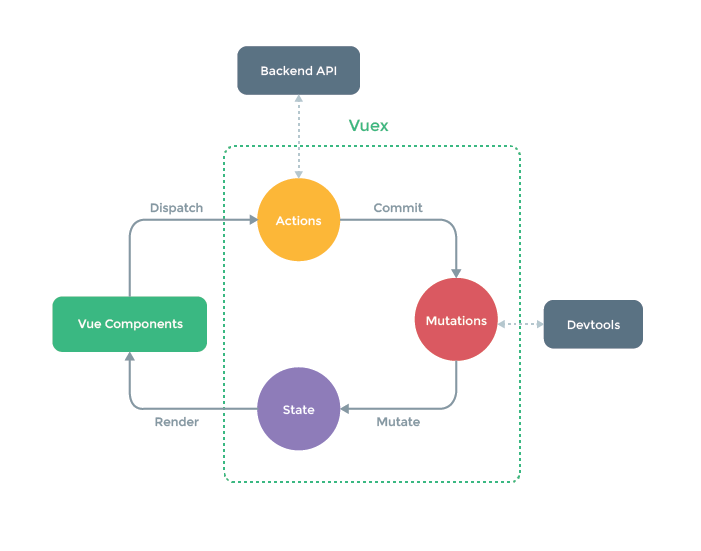
\includegraphics[width=170mm]{Vuevuex.png}
\end{center}

\section{Pattern di design: DAO}
Componenti View seguono il pattern Data Access Object : in questo pattern solo alcuni oggetti possono leggere e scrivere dati su file (o su database) e il loro compito e' fornire un'interfaccia per interagire con i dati/registrazione/visualizzazione...


\section{Pattern di design: Observer/Iterator}
Observer pattern viene implementata da Vue con delle funzioni(subscribe, listen, onclick, onChange) fornite dalle librerie in cui la layer ViewModel sa quando l'utente ha interaggito cone la UI di View.Nello stesso modo la pattern Iterator che viene implementata dai linguaggi Typescript e Python.


\chapter{Test}
In questo capitolo verranno spiegate le principali attività di test che sono state effettuate, sarà fornito anche un esempio pratico di una parte di codice utilizzata per testare l'applicazione. In conclusione si descriverà brevemente anche la prova con utente generico e come è risultata utile al miglioramento del software.
 
\section{Unit Tests}
Per testare il sistema sono stati implementati degli unit test per verificare il buon funzionamento di ogni metodo implementato nel modello. Le varie prove sono state effettuate in concomitanza con lo sviluppo del progetto, in particolare è stato testato ogni metodo dele componenti di visualizzazione di dati,e di singleton class che sono vitali per lo software con il framework JestJs che permette di creare metodi di testing e anche di fare mount di prop components che si dedicano esclusivamente alle operazioni di testing delle componenti originali.Di seguito alcuni esempi:
\begin{figure}[htpb!] 
	\section{Unit test che richiede di definire oggetti di jests}
	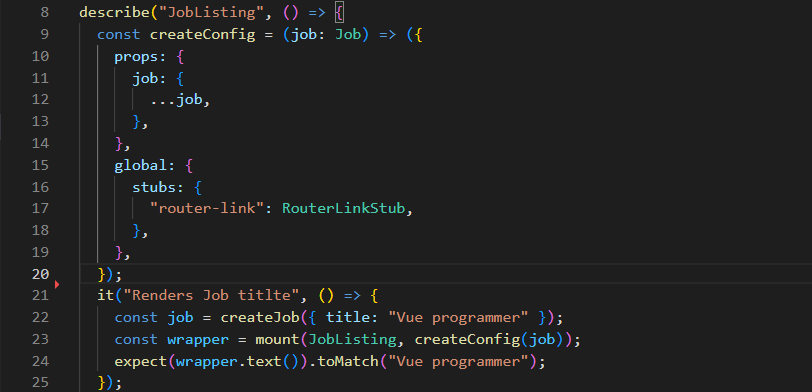
\includegraphics{testWithJestObjects.png}
\end{figure}

\begin{figure}[htpb!] 
	\section{Unit Test getters}
	\centering 
	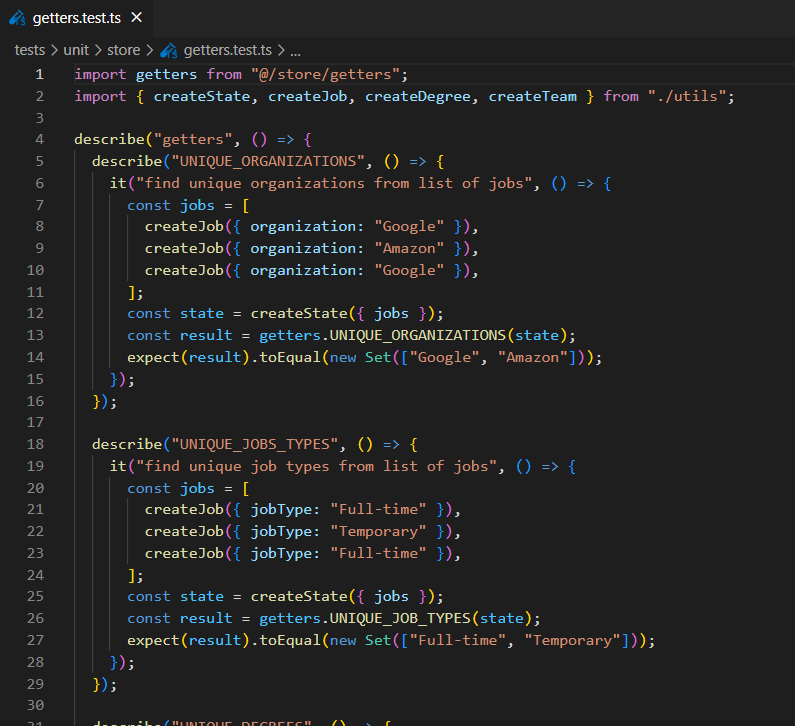
\includegraphics{getterTestExample.png}
\end{figure}

\begin{figure}[htpb!] 
	\section{All Unit Tests passing}
	\includegraphics{allTestUnits.png}
\end{figure}
\begin{figure}[htpb!] 
	\section{Api testing}
	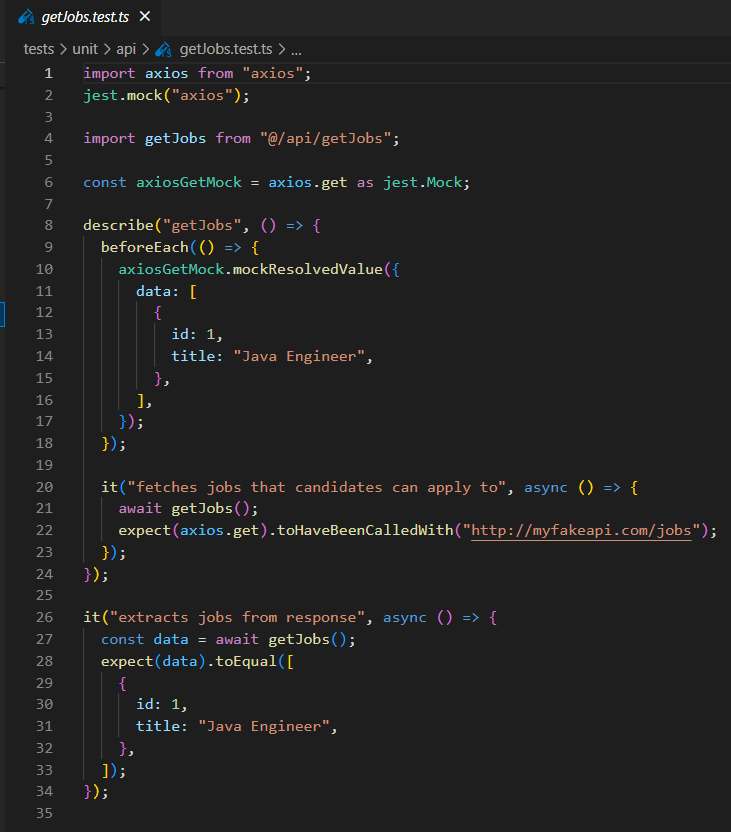
\includegraphics{getJobTest.png}
\end{figure}



\section{Test con utente generico}
Il software è stato presentato ad utenti esterni non a conoscenza della struttura implementativa dell'applicazione, non è stata fornita loro alcun tipo di guida di modo da poter verificare, oltre che la corretta esecuzione del programma, anche l'intuitività dell'interfaccia grafica. Per quanto riguarda la parte funzionale, non sono stati riscontrati problemi rilevanti.
Grazie a questo tipo di test abbiamo inoltre compreso come rendere il sistema più "tollerante" agli inserimenti errati degli filtri di digitare gli spazi in alcune InputField che il sistema non riusciva a gestire se l'input non era inserito correttamente Mentendo la possibilita di correzie di lettere e eliminazioni di spazzi inutili. Dopo queste correzioni è stata riproposta la possibilità all'utente generico di riutilizzare e quindi rivalutare l'applicazione, nella seconda fase di test il tempo di utilizzo da parte di quest'ultimo si è ridotto notevolmente testimoniando il fatto di un miglioramento della struttura grafica.


\end {document}
